\chapter{Pequeños interruptores automáticos}
\section{Características básicas}
Son dispositivos modulares que trabajan a una tensión nominal de 230 o 400V que puede ser utilizar por personal no experto. Recibe distintas denominaciones:
\begin{itemize}
	\item Interruptores automáticos modulares
	\item Magneto-térmicos(relé magnético + relé térmico)
	\item Pequeños interruptores automáticos o MCB (MiniatureCircuitBreaker)
\end{itemize}

Son dispositivos donde su calibre o intensidad asignada están normalizados (son los valores que soportan cables de distintas secciones) con los siguientes valores: 6A, 10A, 16A, 20A, 25A, 32A, 40A, 50A, 63A, 80A, 100A y 125A ajustados a una temperatura de 30$^\circ$C.
\newline

Como la temperatura de trabajo puede variar se emplean tablas para corregir la intensidad asignada y así asegurar que no se dé el disparo térmico en condiciones nominales.
\begin{table}[H]
	\centering
	\begin{tabular}{|c|c|c|c|c|c|c|c|c|c|}
		\hline
		\textbf{Cal. (A)} & \textbf{20°C} & \textbf{25°C} & \textbf{30°C} & \textbf{35°C} & \textbf{40°C} & \textbf{45°C} & \textbf{50°C} & \textbf{55°C} & \textbf{60°C} \\ \hline
		1  & 1.05 & 1.02 & 1.00 & 0.98 & 0.95 & 0.93 & 0.90 & 0.88 & 0.85 \\ \hline
		2  & 2.08 & 2.04 & 2.00 & 1.96 & 1.92 & 1.88 & 1.84 & 1.80 & 1.74 \\ \hline
		3  & 3.18 & 3.09 & 3.00 & 2.91 & 2.82 & 2.70 & 2.61 & 2.52 & 2.43 \\ \hline
		4  & 4.24 & 4.12 & 4.00 & 3.88 & 3.76 & 3.64 & 3.52 & 3.36 & 3.24 \\ \hline
		6  & 6.24 & 6.12 & 6.00 & 5.88 & 5.76 & 5.64 & 5.52 & 5.40 & 5.30 \\ \hline
		10 & 10.6 & 10.3 & 10.0 & 9.70 & 9.30 & 9.00 & 8.60 & 8.20 & 7.80 \\ \hline
		16 & 16.8 & 16.5 & 16.0 & 15.5 & 15.2 & 14.7 & 14.2 & 13.8 & 13.3 \\ \hline
		20 & 21.0 & 20.6 & 20.0 & 19.4 & 18.9 & 18.4 & 17.8 & 17.4 & 16.8 \\ \hline
		25 & 26.2 & 25.7 & 25.0 & 24.2 & 23.7 & 23.0 & 22.2 & 21.5 & 20.7 \\ \hline
		32 & 33.5 & 32.9 & 32.0 & 31.4 & 30.4 & 29.8 & 28.8 & 28.2 & 27.5 \\ \hline
		40 & 42.0 & 41.2 & 40.0 & 38.8 & 37.6 & 36.8 & 35.4 & 34.4 & 33.2 \\ \hline
		50 & 52.5 & 51.5 & 50.0 & 48.5 & 47.4 & 45.5 & 44.0 & 42.5 & 40.5 \\ \hline
		63 & 66.2 & 64.9 & 63.0 & 61.1 & 58.0 & 56.7 & 54.2 & 51.7 & 49.2 \\ \hline
	\end{tabular}
\end{table}

Además de la temperatura si hay aparatos contiguos es necesario aplicar otro factor de corrección. Además, si se disponen en dos filas la intensidad nominal se reduce otro 25\% y si son tres filas un30\%.
\begin{table}[H]
	\centering
	\begin{tabular}{|c|c|c|c|c|}
		\hline
		\textbf{Nº de aparatos contiguos} & \textbf{Siemens} & \textbf{Hager} & \textbf{Terasaki} & \textbf{ABB} \\ \hline
		1  & 1    & 1    & 1    & 1    \\ \hline
		2  & 0.90 & 1    & 0.90 & 0.95 \\ \hline
		3  & 0.90 & 0.95 & 0.84 & 0.90 \\ \hline
		4  & 0.88 & 0.90 & 0.82 & 0.86 \\ \hline
		5  & 0.88 & 0.90 & 0.80 & 0.82 \\ \hline
		6  & 0.88 & 0.85 & 0.79 & 0.795 \\ \hline
		7  & 0.85 & 0.85 & 0.78 & 0.78  \\ \hline
		8  & 0.85 & 0.85 & 0.76 & 0.77  \\ \hline
		9  & 0.85 & 0.85 & -    & 0.76  \\ \hline
		>9 & 0.85 & 0.85 & -    & 0.76  \\ \hline
	\end{tabular}
\end{table}



\subsection{Capacidad o poder de corte}
Se define la capacidad de corte asignado en cortocircuito la máxima intensidad de cortocircuito que es capaz de abrir el interruptor automático. \textbf{Se denota con $I_{cn}$}.
\newline

El fabricante proporciona el valor eficaz del poder de corte máximo. Tiene los valores normalizados de 3kA, 4,5kA, 6kA, 10kA, 15kA, 20kA y 25 kA.
\newline

Tal como se vio en temas anteriores como el corte del cortocircuito depende de la tensión el valor de la intensidad se $\textbf{tiene que proporcionar}$ con la tensión, frecuencia y factor de potencia asignados. Para obtener este valor no se requiere el ensayo de calentamiento.
\newline

Para obtener este valor se emplean las hipótesis de cálculo mencionadas en anteriores temas y aunque en la realidad es poco probable que sean tan desfavorables siempre prima la precaución. Aún así, es muy probable que la corriente en el cortocircuito sea menor.

\subsection{Poder de corte de servicio en cortocircuito}
Se define como el poder de corte de un ciclo de apertura-cierre / apertura-cierre /apertura cierre, es decir, el interruptor automático debe efectuar tres rupturas sucesivas de la corriente. \textbf{Se denota con $I_{cs}$}.
\newline

Se debe verificar mediante ensayo de calentamiento y se expresa como un \% de $I_{cn}$.
\begin{table}[H]
	\centering
	\begin{tabular}{|c|c|}
		\hline
		\textbf{Icn (kA)} & \textbf{Factor de Corrección (k)} \\ \hline
		$\leq 6000 \, \text{A}$    & 1    \\ \hline
		Valores intermedios & 0.75 \\ \hline
		$> 10000 \, \text{A}$  & 0.5   \\ \hline
	\end{tabular}
\end{table}
\subsection{Curvas de disparo}
\begin{figure}[H]
	\centering
	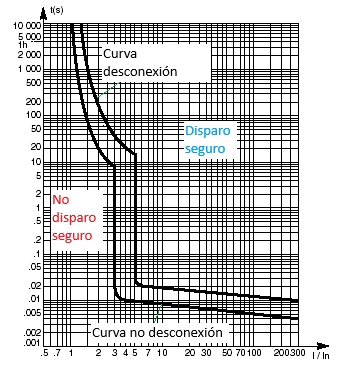
\includegraphics[width=0.5\linewidth]{Images/12}
	\label{fig:12}
\end{figure}

Esta curva se puede describir mediante la siguiente tabla donde se puede ver que existen distintas curvas en función del tipo de disparo deseado:
\begin{table}[H]
	\centering
	\begin{tabular}{|c|c|c|c|}
		\hline
		\textbf{Curva} & \textbf{Intensidad ensayo} & \textbf{Límites de tiempo} & \textbf{Disparo} \\ \hline
		B, C, D & $1.13 \, I_n$ & $t \geq 1 \, \text{h}$ & No \\ \hline
		B, C, D & $1.45 \, I_n$ & $t < 1 \, \text{h}$ & Sí \\ \hline
		B, C, D & $2.55 \, I_n$ & $1 \, \text{s} < t < 60 \, \text{s}$ & Sí \\ \hline
		\color{red}
		B      &\color{red} $3 \, I_n$    &\color{red} $t \geq 0.1 \, \text{s}$ &\color{red} No \\ \hline
		\color{red}C      & \color{red}$5 \, I_n$    &\color{red} $t \geq 0.1 \, \text{s}$ &\color{red} No \\ \hline
		\color{red} D      &\color{red} $10 \, I_n$   &\color{red} $t \geq 0.1 \, \text{s}$ &\color{red} No \\ \hline
				\color{blue}
		B      &\color{blue} $5 \, I_n$    &\color{blue} $t < 0.1 \, \text{s}$ &\color{blue} Sí \\ \hline
		\color{blue} C      &\color{blue} $10 \, I_n$   &\color{blue} $t < 0.1 \, \text{s}$ &\color{blue} Sí \\ \hline
		\color{blue}D      &\color{blue} $14 \, I_n$   & \color{blue}$t < 0.1 \, \text{s}$ & \color{blue} Sí \\ \hline
	\end{tabular}
\end{table}
				\color{black}

En la tabla anterior se observa como la única diferencia entre las curvas es el disparo magnético donde la curva A estaría a la izquierda de la curva B y esta a la izquierda de la curva C.
\newpage
\subsection{Corriente de cortocircuito limitada}
Los fabricantes también proporcionan el valor de la curva de corriente limitada para conocer la eficacia de la ruptura:
\begin{figure}[H]
	\centering
	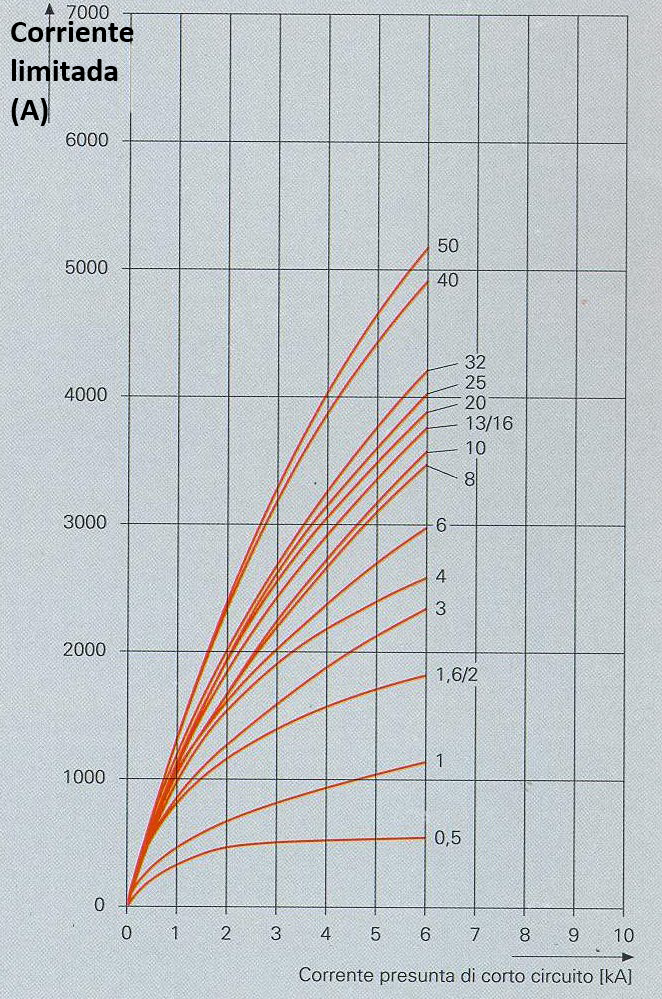
\includegraphics[width=0.3\linewidth]{Images/13}
	\label{fig:13}
\end{figure}
\subsection{Clases de limitación de la energía}
En función de la clase de limitación de la energía la protección tiene una clase u otra:
\begin{table}[H]
	\centering
	\begin{adjustbox}{width=1\textwidth}

	\begin{tabular}{|c|c|c|c|c|c|}
		\hline
		\multirow{2}{*}{\textbf{Capacidad de cortocircuito asignada (A)}} & \multicolumn{5}{c|}{\textbf{Tipo C}} \\ \cline{2-6} 
		& \textbf{Clase 1} & \multicolumn{4}{c|}{\textbf{Clase 3}} \\ \cline{2-6} 
		& $\leq 63 \, \text{A}$ & $\leq 16 \, \text{A}$ & $20 \, \text{A}, 25 \, \text{A}, 32 \, \text{A}$ & $40 \, \text{A}$ & $50 \, \text{A}, 63 \, \text{A}$ \\ \hline
		3000  & No hay límites definidos &17000 & 20000 & 24000 & 30000 \\ \hline
		4500  & - &28000 & 37000 & 45000 & 55000 \\ \hline
		6000  & - & 40000 & 52000 & 63000 & 75000 \\ \hline
		10000 & - &80000 & 100000 & 120000 & 145000 \\ \hline
	\end{tabular}
		
	\end{adjustbox}
\end{table}
\subsection{Panel frontal}
\begin{figure}[H]
	\centering
	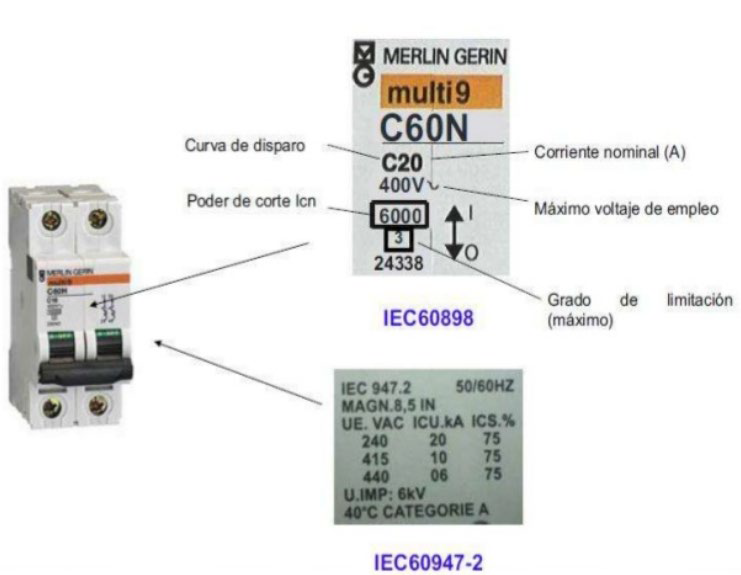
\includegraphics[width=0.7\linewidth]{Images/14}
	\label{fig:14}
\end{figure}
\subsection{Número de polos}
Los dispositivos de corte unipolares están prohibidos. Por tanto, existen los dispositivos bipolares 2p (2 polos iguales) o 1p+1N (fase y neutro), tripolares 3p y tetrapolares 4p, 3p+1N o 3p+1/2N (neutro de sección mitad).
\section{Selección de pequeños interruptores automáticos}
\subsection{Normativa y cuestiones generales}
Por normativa todo circuito estará protegido contra los efectos de las sobreintensidades que puedan presentarse en el mismo que pueden estar motivadas por sobrecargas, cortocircuitos o descargas atmosféricas. Para la protección se admiten fusibles e interruptores automáticos.
\newline

El objetivo es proteger todos los conductores activos, \textbf{no las cargas}, solo la instalación eléctrica. Para ello, se sitúan dispositivos de protección en el origen del circuitos y en los puntos donde disminuya la intensidad por un cambio de sección.
\newline

En el cuadro general de mando y protección (CGMP) se coloca en el inicio un interruptor general automático (IGA), un interruptor diferencial general (DDR), dispositivos de protección contra sobreintensidadespara cada circuito interior y dispositivos de protección contra sobretensiones.
\subsection{Partes protegidas de una instalación}
Cada uno de los circuitos esta protegido por el interruptor de su mismo color. El interruptor general de un CAMP puede ser un interruptor automático o un interruptor seccionador de corte en carga (lo protege la protección anterior).
\begin{figure}[H]
	\centering
	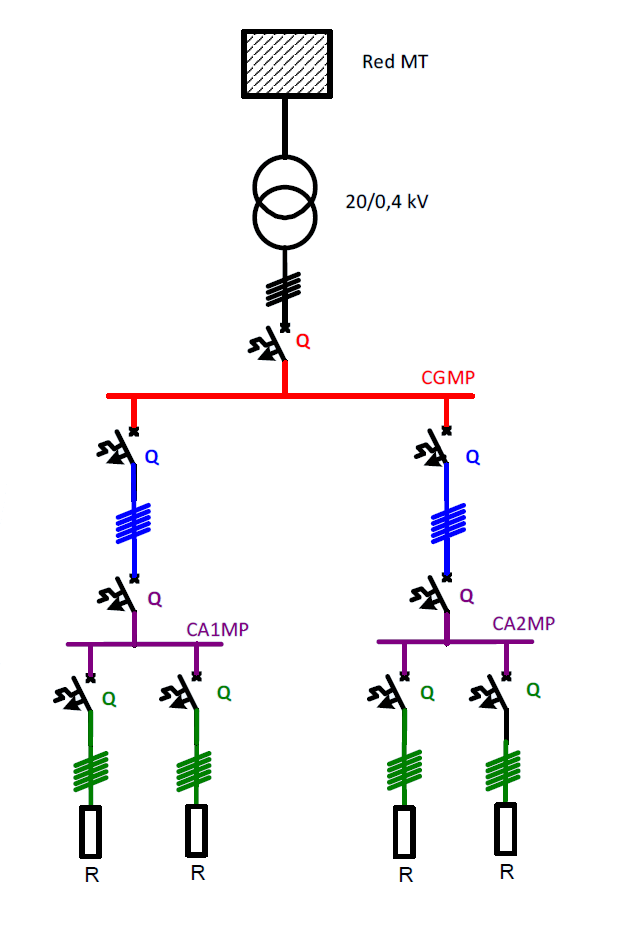
\includegraphics[width=0.7\linewidth]{Images/15}
	\label{fig:15}
\end{figure}

\subsection{Tensión asignada}
La tensión asignada de la instalación debe ser mayor o igual que la nominal. 
\begin{itemize}
	\item Los interruptores automáticos de tensión asignada 230V pueden ser 1p+N o 2p. Debe conectarse a un circuito monofásico fase a neutro de tensión nominal 230 V
	\item Los interruptores automáticos de tensión asignada 230V solo pueden ser 2p. Puede conectarse a un circuito monofásico fase a neutro de tensión nominal 230 V o a un circuito bifásico de 400 V
	\item Interruptores automáticos tripolares deben tener los tres polos protegidos 3p. Debe tener tensión asignada 400 V o superior para conectarse a un circuito trifásico de 400 V
	\item Interruptores automáticos tetrapolarespueden tener tres (3p + N) o cuatro polos protegidos (4p). Debe tener tensión asignada 400 V o superior para conectarse a un circuito trifásico de 400 V
\end{itemize}


\subsection{Número de polos}
En la siguiente tabla se pude ver si una de las fases necesita un dispositivo de protección o detección sobre el conductor correspondiente (P)
\begin{table}[H]
	\centering
	\begin{tabular}{|c|c|c|c|c|c|c|c|c|c|c|c|c|c|c|c|}
		\hline
		\multirow{3}{*}{\textbf{Esquemas}} &	\multicolumn{8}{c|}{3F+N}& \multicolumn{3}{c|}{3F} & \multicolumn{2}{c|}{2F}& \multicolumn{2}{c|}{F+N}\\ \cline{2-9} 
		 & \multicolumn{4}{c|}{$S_N\ge S_F$}& \multicolumn{4}{c|}{$S_N<S_F$}&\multicolumn{3}{c|}{} & \multicolumn{2}{c|}{}& \multicolumn{2}{c|}{}\\ \cline{2-16} 
		& F & F & F & N & F & F & F & N & F & F & F  & F & F & N & F \\ \hline
		\textbf{TN-C} & P & P &P  & - & P & P & P & -  & P & P & P & P & P  & P & - \\ \hline
		\textbf{TN-S} & P & P &P  & - & P & P & P & P  & P & P & P & P & P  & P &- \\ \hline
		\textbf{TT}   & P & P &P  & - & P & P & P & P  & P & P & P & P & P  & P &- \\ \hline
		\textbf{IT}   & P & P & P & P & P & P & P & P  & P & P & P & P & P  & P &P \\ \hline
	\end{tabular}
\end{table}

Según la ITC-BT-19 se debe justificar por cálculos las secciones de neutro distintas a las secciones de fase que viene dada por:
\begin{itemize}
	\item Cargas monofásicas
	\item Falta de equilibrio entre las cargas monofásicas
	\item Cargas no lineales (distorsión armónica)
\end{itemize}

Si la sección de neutro es menor siempre ha de tener una protección distinta al poder estar en condiciones de falta el cable sin que salten las protecciones (distinta corriente en función de la sección).
\newline

Existen dos tipos de polo no protegido:
\begin{enumerate}
	\item Polo no protegido: Sin relé de disparo pero con poder de corte
	\item Polo seccionador de neutro: Sin poder de corte. Debe abrir después y cerrar antes que los polos protegidos.
\end{enumerate}
\subsection{Intensidad asignada}
Se debe cumplir que:
\begin{equation}
	I_L < I_{NQ} < I_Z
\end{equation}

Donde $I_L$ es la intensidad de las cargas, $I_{NQ}$ la intensidad asignada y $I_z$ la intensidad admisible del cable. Se debe tener en cuenta para el cálculo de la intensidad de las cargas que:
\begin{itemize}
	\item Si hay un motor su potencia $1,25P_N$
	\item Si más de un motor su potencia $\sum P_N+1,25P_{N_{Mayor}}$
	\item Máquinas elevadoras $1,3P_N$
	\item Lámparas de descarga $1,8P_N$
\end{itemize}

A esta intensidad asignada de la protección es necesario aplicar una corrección por temperatura.
\subsection{Poder de corte asignado}
El interruptor automático debe ser capaz de abrir cualquier corriente de cortocircuito en el punto de su instalación. Por tanto el poder de corte asignado $I_{cn}>I_{k_{max}}$. Mientras que el poder de corte en cortocircuito ($I_{cs}$) se elige como valor el del cortocircuito más probable. Si es una instalación crítica debe ser mayor que la corriente de cortocircuito máxima.
\newline

En el interruptor automático general: la intensidad de cortocircuito que debe abrir sólo depende del tipo de cortocircuito. No depende del punto del cuadro donde se produce la falta.
\subsection{Umbral de disparo magnético}
Se elige la curva de tal manera que se cumpla que 
\begin{equation}
	\dfrac{I_{arranque}}{I_n}< n < \dfrac{I_{k_{min}}}{I_n}
\end{equation}
\begin{table}[H]
	\centering
	\begin{tabular}{|c|c|c|c|}
		\hline
		\textbf{Múltiplo de In} & \textbf{Curva B} & \textbf{Curva C} & \textbf{Curva D} \\ \hline
		n\textsubscript{min} & 3 & 5 & 10 \\ \hline
		n\textsubscript{max} & 5 & 10 & 14 \\ \hline
	\end{tabular}
\end{table}




